
\chapter{系统实现和实验结果}
\label{chap:experiment}

\section{系统具体实现}
\label{sec:implementation}
我们采用Scala语言来搭建我们的系统。Scala是一种运行在JVM上的静态语言,支持函数式、
面向对象等多种编程范式,可以和Java代码无缝地进行交互。目前Scala还处于不断发展中,
新版本不向后兼容,我们的系统在Scala 2.10上可以编译通过。在工程管理上,我们使
用sbt管理Scala代码的编译和依赖关系。

在系统的实现中我们还使用了许多第三方库,主要有:
\begin{itemize}
\item 日志系统:基于twitter公司开源的util包,地址在
  \url{https://github.com/twitter/util}。
\item 网页字符集检测:ICU4J,地址在\url{http://site.icu-project.org},这是一
  套UNICODE相关的工具集,提供了较好的字符集编码检测功能,我们用于检测中文网页的字
  符集。
\item HTML解析器:jsoup,地址在\url{http://jsoup.org},是一个用Java语言实现
  的HTML解析器,用于DOM Tree的构建和节点内容的抽取。
\item Actor库:Akka。在第~\ref{chap:cluster}章中已经做了介绍。
\end{itemize}
\section{实验演示系统}
\label{sec:demo}
为了直观地显示网页模板的匹配效果,我们基于Play! Framework的Web开发框架实现了一
个Web Service,用于实验的演示。该Web Service的工作原理
如\reffig{experiment:fig:demo}所示。
\begin{figure}
  \centering
  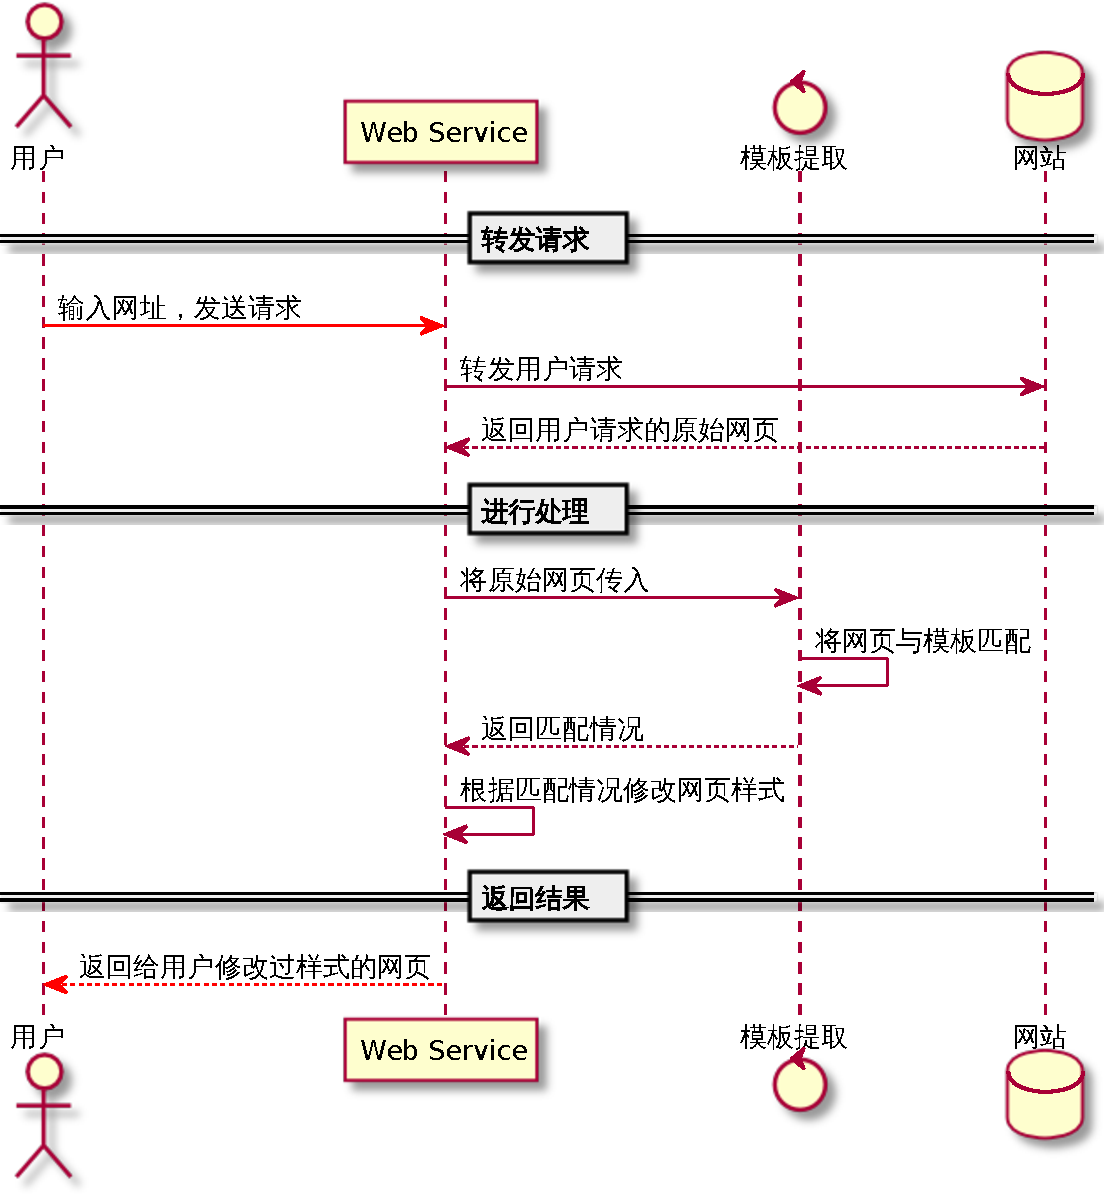
\includegraphics[width=0.75\textwidth]{experiment06/demo}
  \caption{Web Service工作原理}
  \label{experiment:fig:demo}
\end{figure}

用户只需要输入一个需要和系统的模板进行匹配的网页的URL,系统将返回一个修改过样式的
新的网页,使得原网页和模板的匹配情况可以从浏览器中直观地看到。
% TODO: 实验演示的效果如\reffig{experiment:fig:demoresult}所示
% \begin{figure}
%   \centering
%   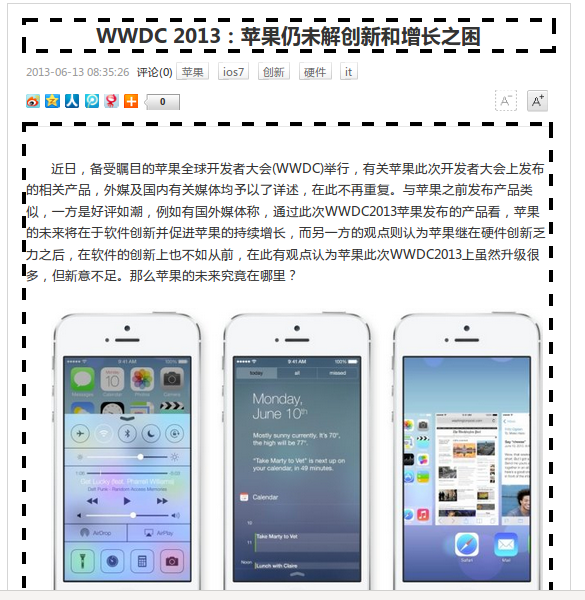
\includegraphics[width=0.5\textwidth]{experiment06/demoresult}
%   \caption{实验演示系统效果}
%   \label{experiment:fig:demoresult}
% \end{figure}

\section{实验数据和实验环境}
\label{sec:dataenv}
实验数据的概况如表~\ref{experiment:tab:overview}所示。
\begin{table}
  \centering
% BEGIN RECEIVE ORGTBL 实验数据概况
\begin{tabular}{llll}
\hline
 & blog & news & other \\
\hline
文件个数 & 59998 & 81561 & 183635 \\
总大小 & 5.4G & 7.9G & 18G \\
来源 & blog.sina.com.cn &  news.xxx.com &  \\
\hline
\end{tabular}
% END RECEIVE ORGTBL 实验数据概况
  \caption{实验数据概况}
  \label{experiment:tab:overview}
\end{table}
\begin{comment}
#+ORGTBL: SEND 实验数据概况 orgtbl-to-latex :splice nil :skip 0
|----------+------------------+-------+--------|
|          | blog             | news  | other  |
|----------+------------------+-------+--------|
| 文件个数 | 59998            | 81561 | 183635 |
| 总大小   | 5.4G             | 7.9G  | 18G    |
| 来源     | blog.sina.com.cn |       |        |
|----------+------------------+-------+--------|
\end{comment}

以下是我们实验中一些主要参数的的设置情况:
\begin{table}\centering
% BEGIN RECEIVE ORGTBL 参数设置
\begin{tabular}{ll}
聚类相似度阈值 & 0.7\\
训练的样本数 &  \\
用于抽取的数据 &  \\
\end{tabular}
% END RECEIVE ORGTBL 参数设置
\caption{主要参数设置}
\label{experiment:tab:param}
\end{table}
\begin{comment}
#+ORGTBL: SEND 参数设置 orgtbl-to-latex :splice nil :skip 0
| 聚类相似度阈值 |   |
| 训练的样本数   |   |
| 用于抽取的数据 |   |
\end{comment}
\section{实验结果}
\label{sec:results}
我们将分模块进行实验。
\section{结果分析和存在的问题}
\label{sec:analysis}

%%% Local Variables: 
%%% mode: latex
%%% TeX-master: "../main"
%%% End: 
